\begin{subfigures}
	\begin{figure}[!htbp]
		{
		\renewcommand{\arraystretch}{0.1}		
		\centering	
	%	\subfloat[]{
		\begin{tabular}{|p{.5cm} c c|}
			\hline
			&&\\[1em]
			&	\phewon\ 	& \simple \\[1.5em]
			%
			%
			\begin{sideways}{\hspace{3cm} \textbf{All particles}}\end{sideways} \hspace*{-1em}	&		 
			{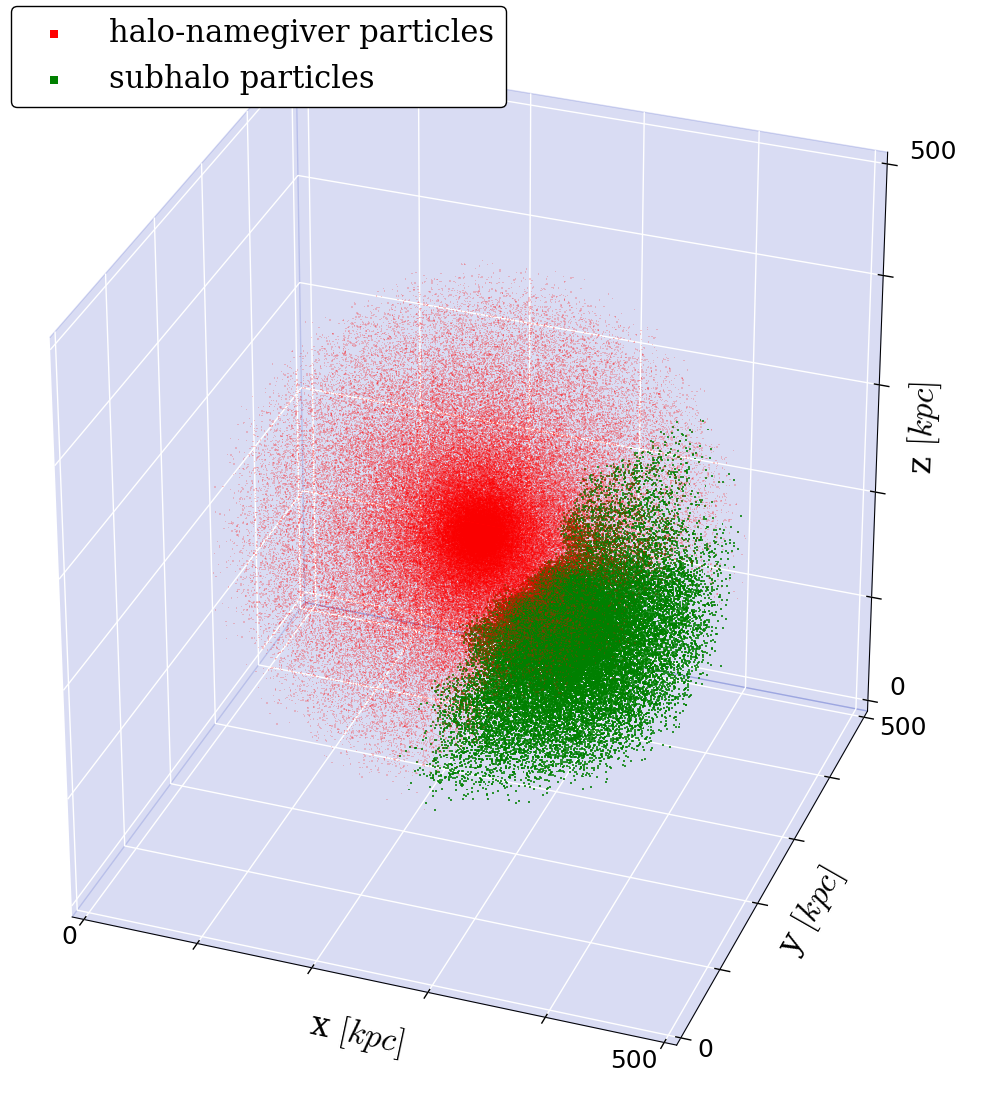
\includegraphics[width = .42\textwidth]{images/dice-two/dice-two-plot-halo1451-phew.png}} \hspace*{-1em} 	& 
			{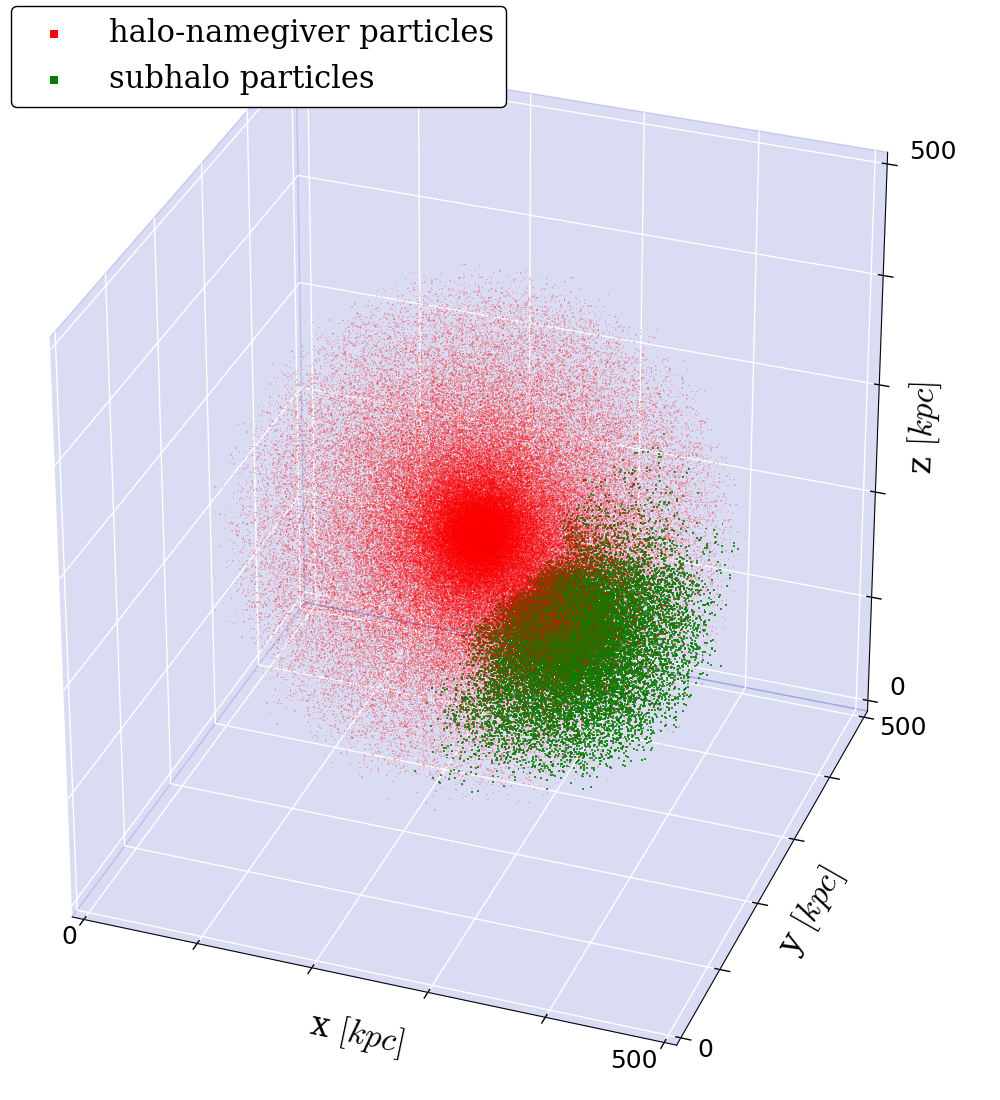
\includegraphics[width = .42\textwidth]{images/dice-two/dice-two-plot-halo1451-nosaddle.png}} \hspace*{-1em}	\\
			%
			%
			\begin{sideways}{ \hspace{.5cm}\textbf{Halo-namegiver particles only} }\end{sideways}	 \hspace*{-1em}			 &			 
			{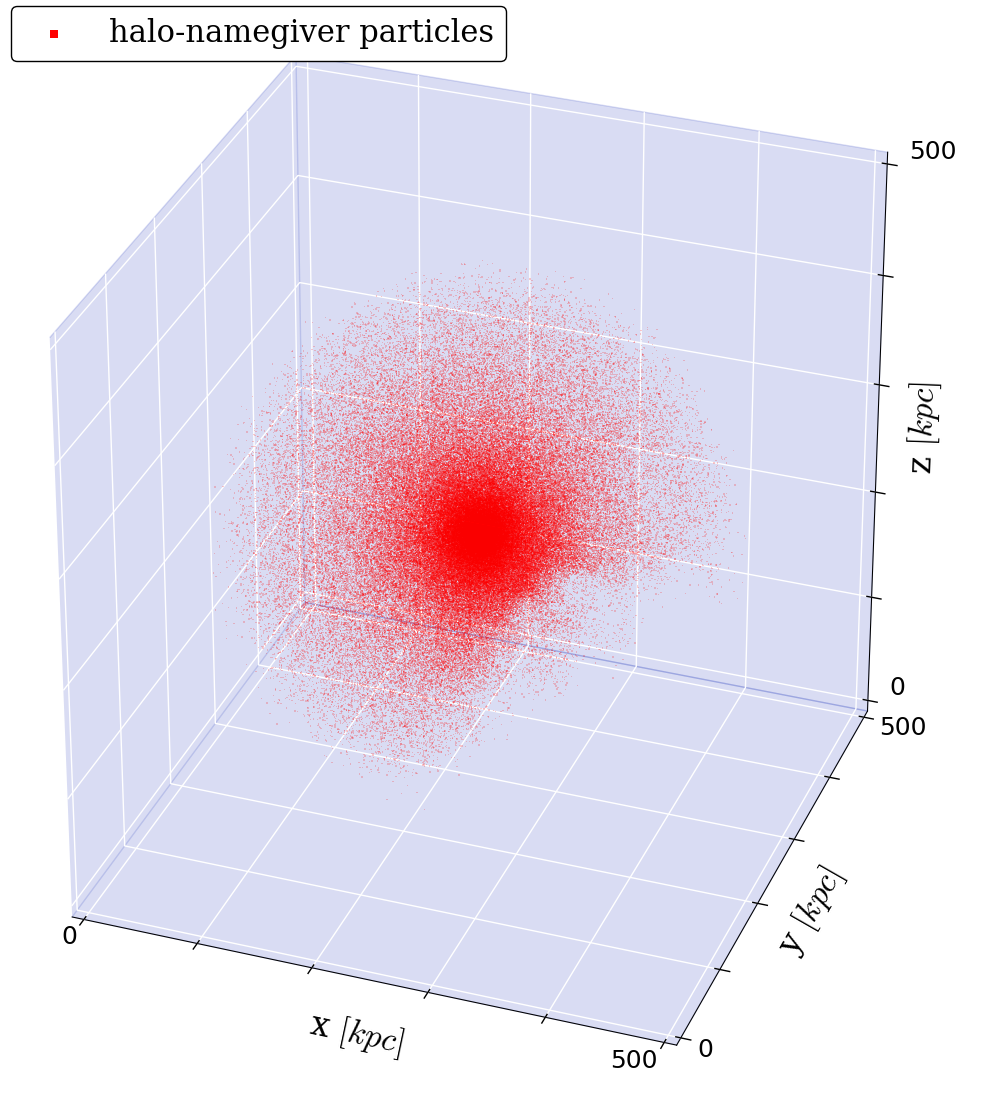
\includegraphics[width = .42\textwidth]{images/dice-two/dice-two-halo-only-phew.png}} \hspace*{-1em} 		&
			{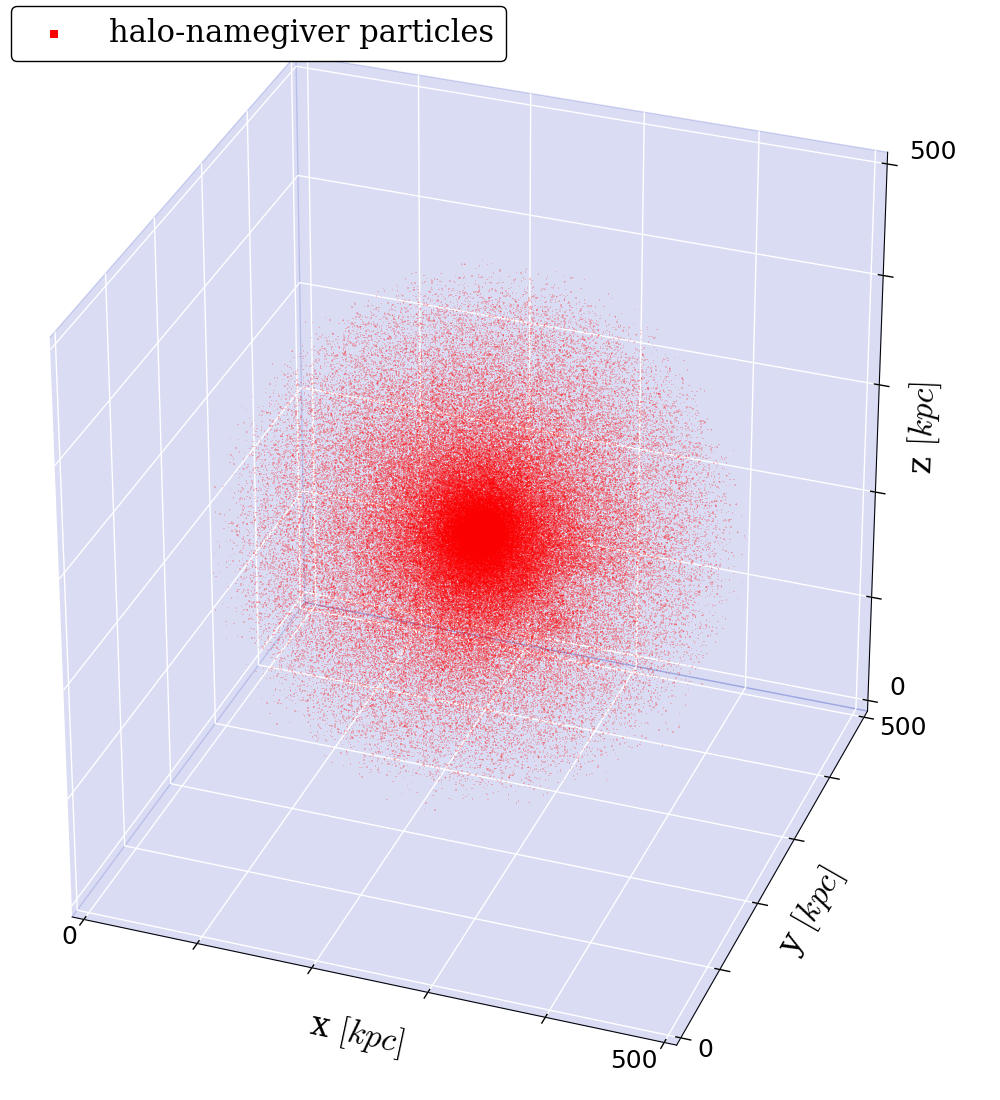
\includegraphics[width = .42\textwidth]{images/dice-two/dice-two-halo-only-nosaddle.png}} \hspace*{-1em}		\\
			%
			%
			\begin{sideways}{ \hspace{2cm}\textbf{Subhalo particles only} }\end{sideways}	 \hspace*{-1em}			 &
			{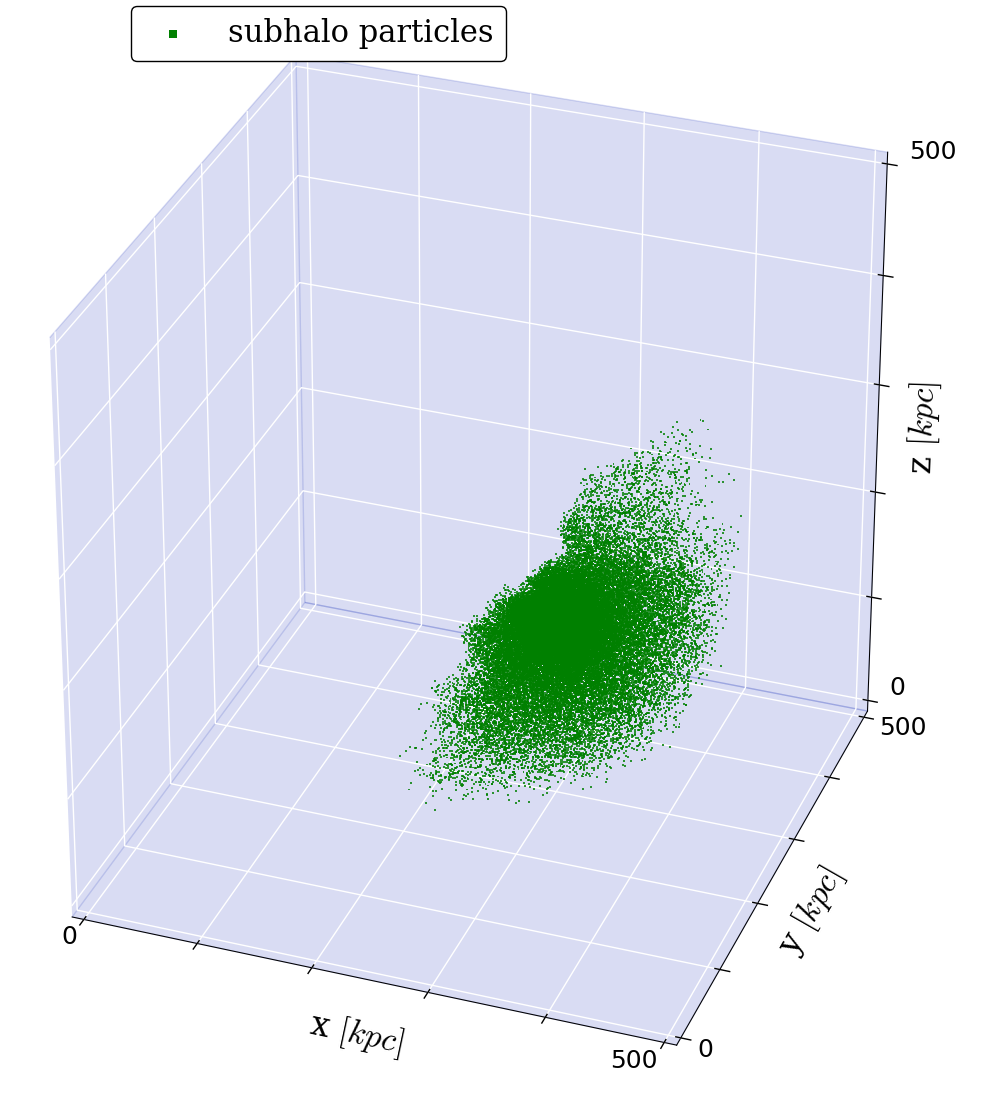
\includegraphics[width = .42\textwidth]{images/dice-two/dice-two-plot-subhalo-phew.png}} &
			{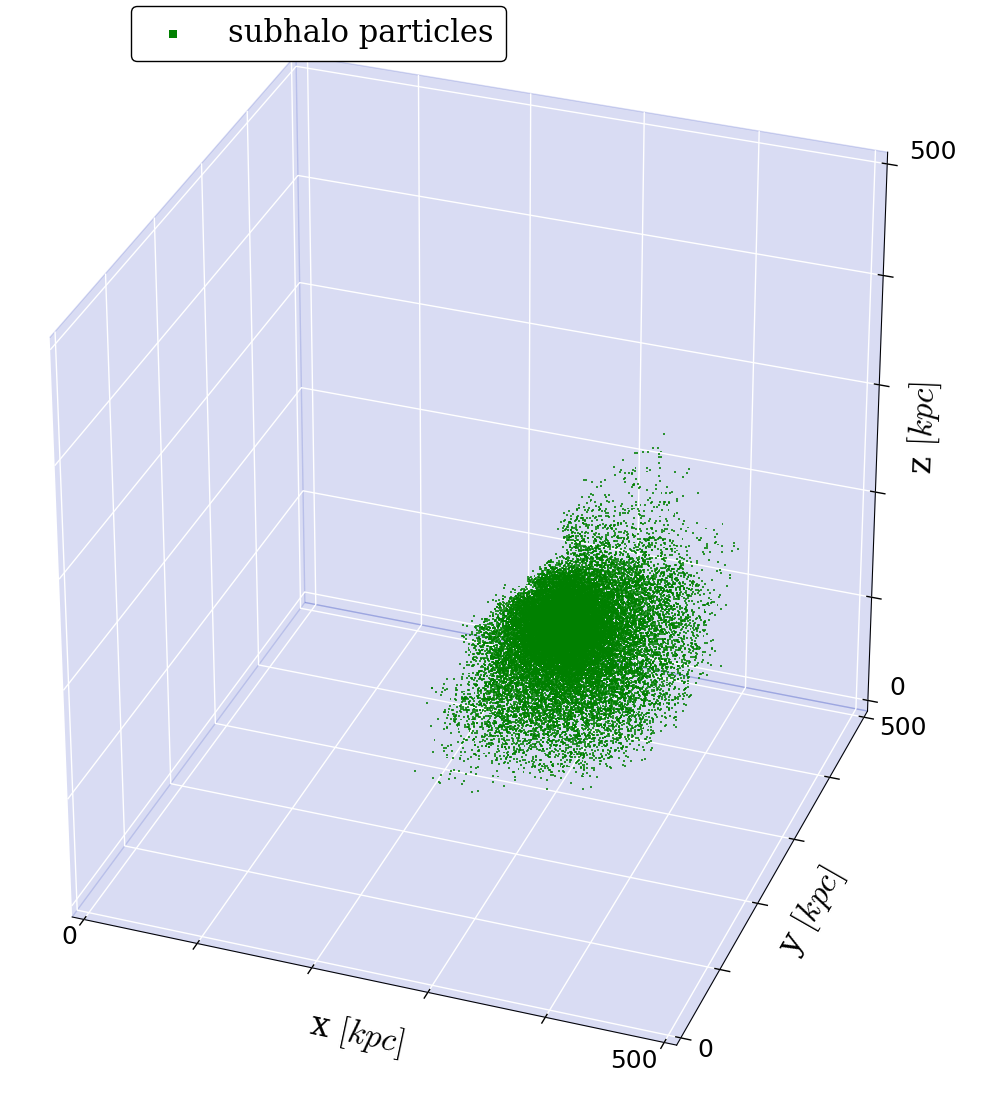
\includegraphics[width = .42\textwidth]{images/dice-two/dice-two-plot-subhalo-nosaddle.png}} \\
			\hline
		\end{tabular}
		\caption{\label{fig:dice_two_results_a}The results of \phewon\ and \simple\ unbinding of the \dt-dataset: All particles, halo-namegiver particles only and subhalo particles only.}
		}
	\end{figure}
%=================================================
%=================================================
%=================================================
	\begin{figure}[!htbp]%\ContinuedFloat
		{
		\renewcommand{\arraystretch}{0.1}
		\centering	
		\begin{tabular}{|p{.5cm} c c|}
			\hline
			&&\\[1em]
			&	\neigh\ 	& \iter \\[1.5em]
			%
			%
			\begin{sideways}{\hspace{3cm} \textbf{All particles}}\end{sideways} \hspace*{-1em}	&		 
			{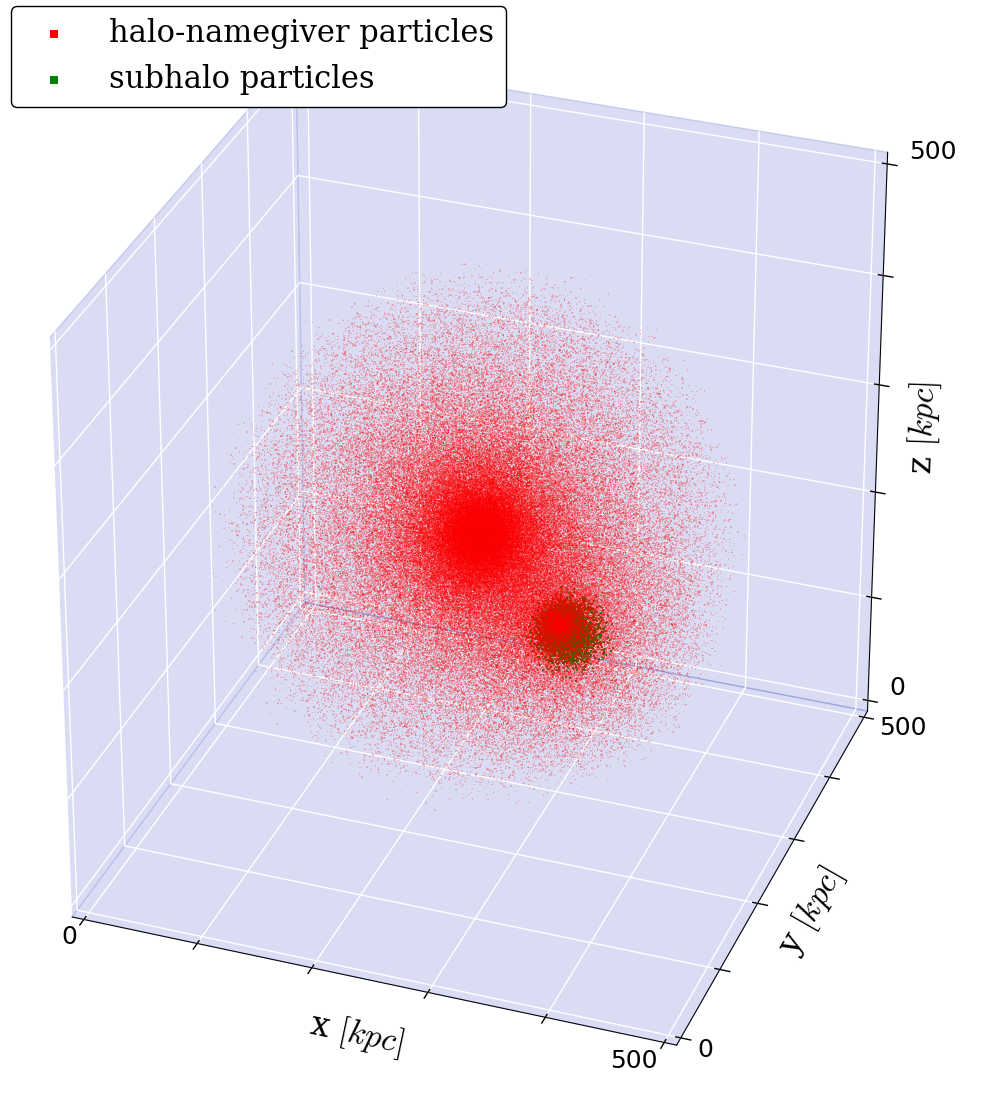
\includegraphics[width = .42\textwidth]{images/dice-two/dice-two-plot-halo1451-saddle.png}} \hspace*{-1em} 	& 
			{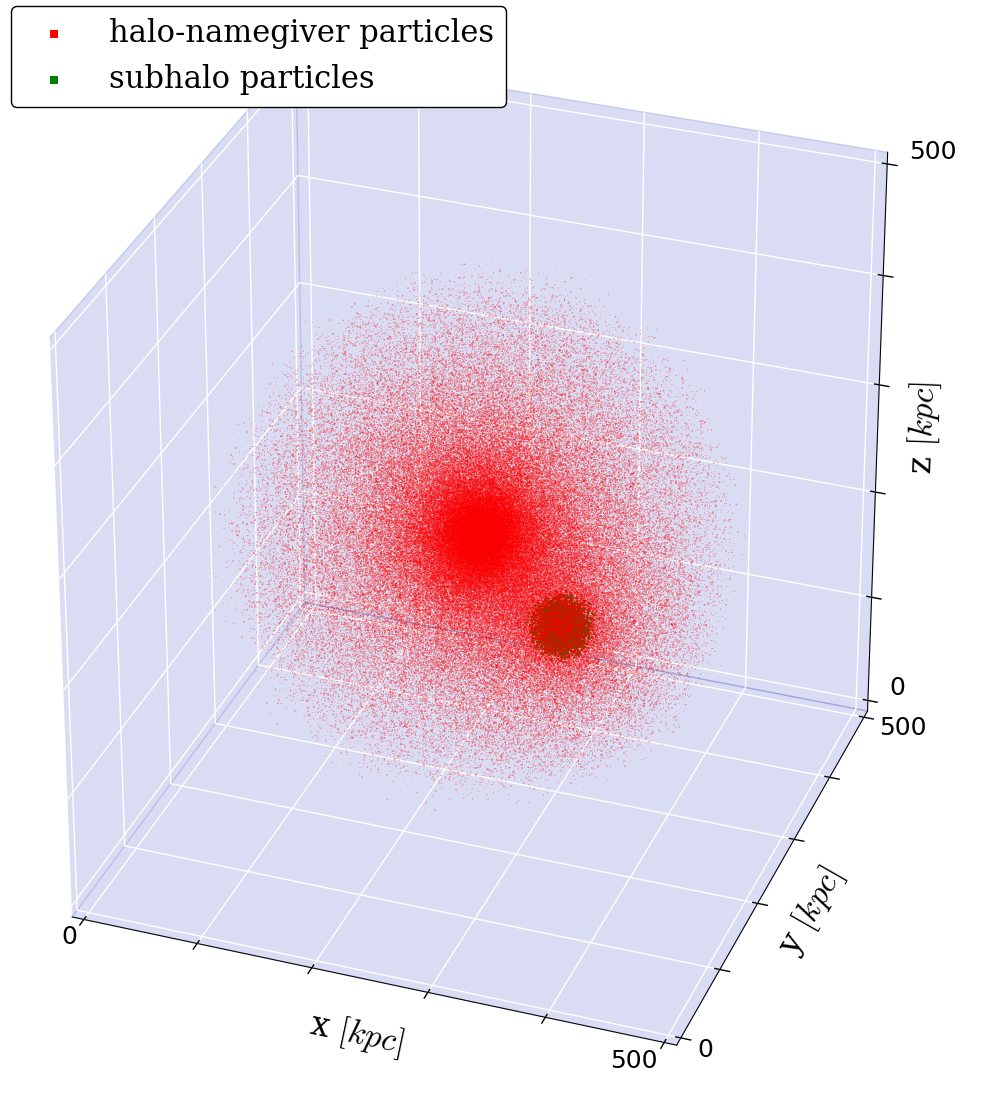
\includegraphics[width = .42\textwidth]{images/dice-two/dice-two-plot-halo1451-iter.png}} \hspace*{-1em}	\\
			%
			%
			\begin{sideways}{ \hspace{.5cm}\textbf{Halo-namegiver particles only} }\end{sideways}	 \hspace*{-1em}			 &			 
			{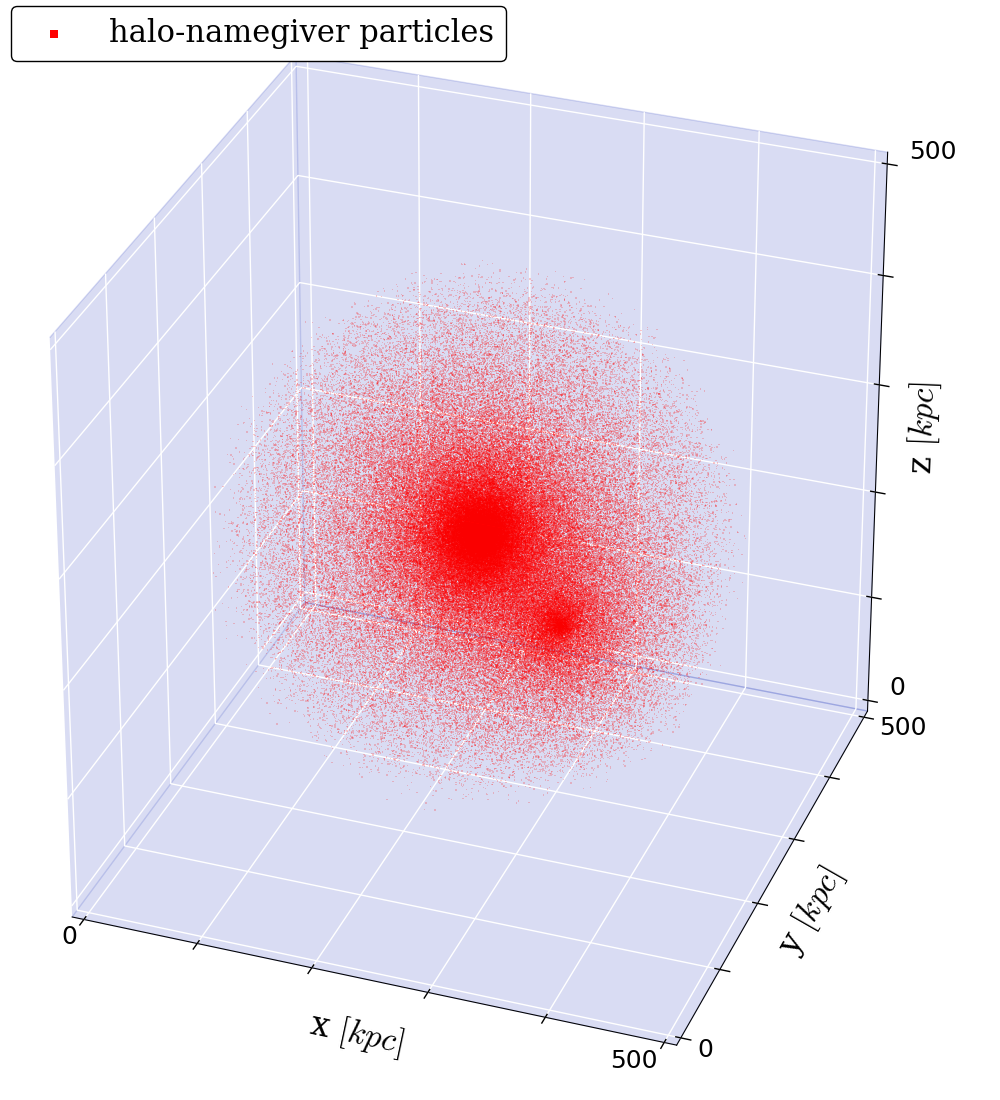
\includegraphics[width = .42\textwidth]{images/dice-two/dice-two-halo-only-saddle.png}} \hspace*{-1em} 		&
			{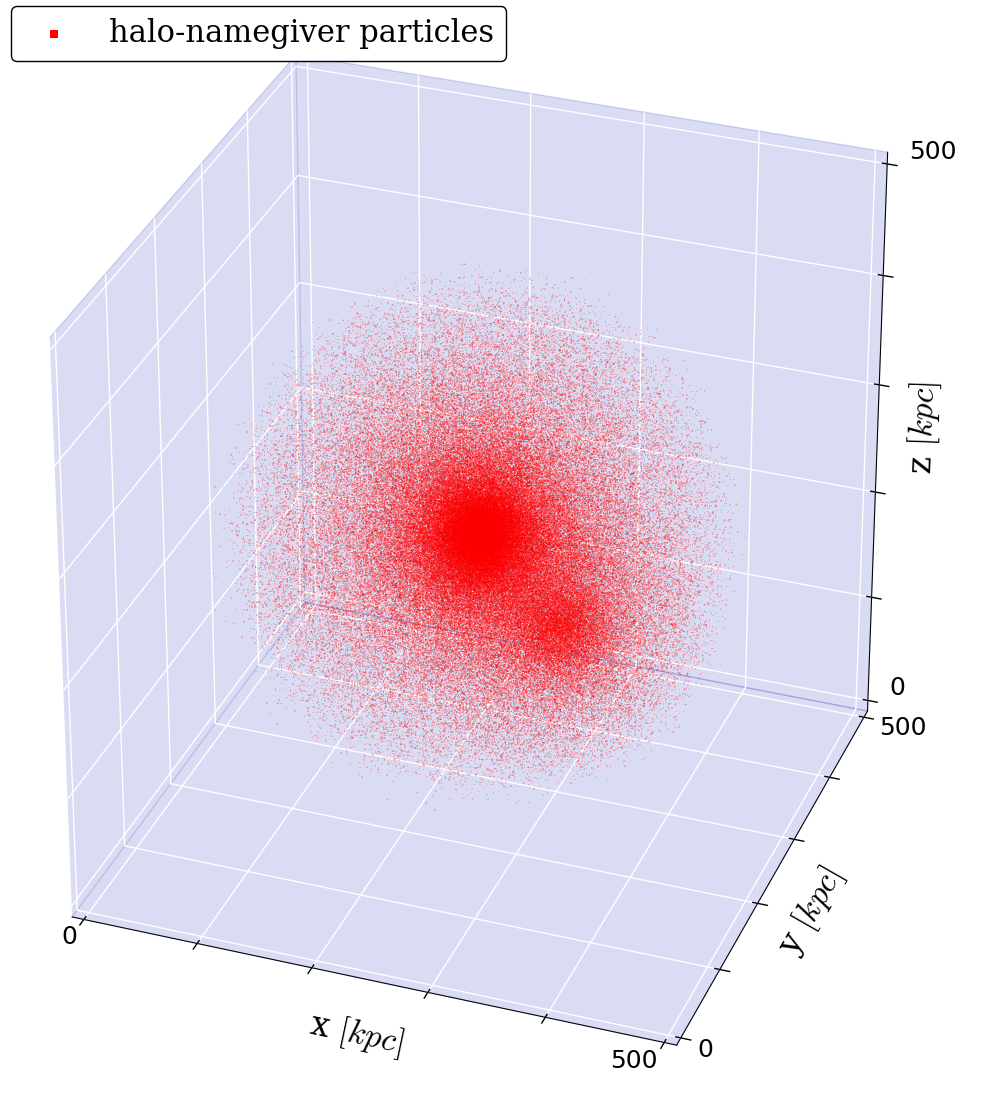
\includegraphics[width = .42\textwidth]{images/dice-two/dice-two-halo-only-iter.png}} \hspace*{-1em}		\\
			%
			%
			\begin{sideways}{ \hspace{2cm}\textbf{Subhalo particles only} }\end{sideways}	 \hspace*{-1em}			 &
			{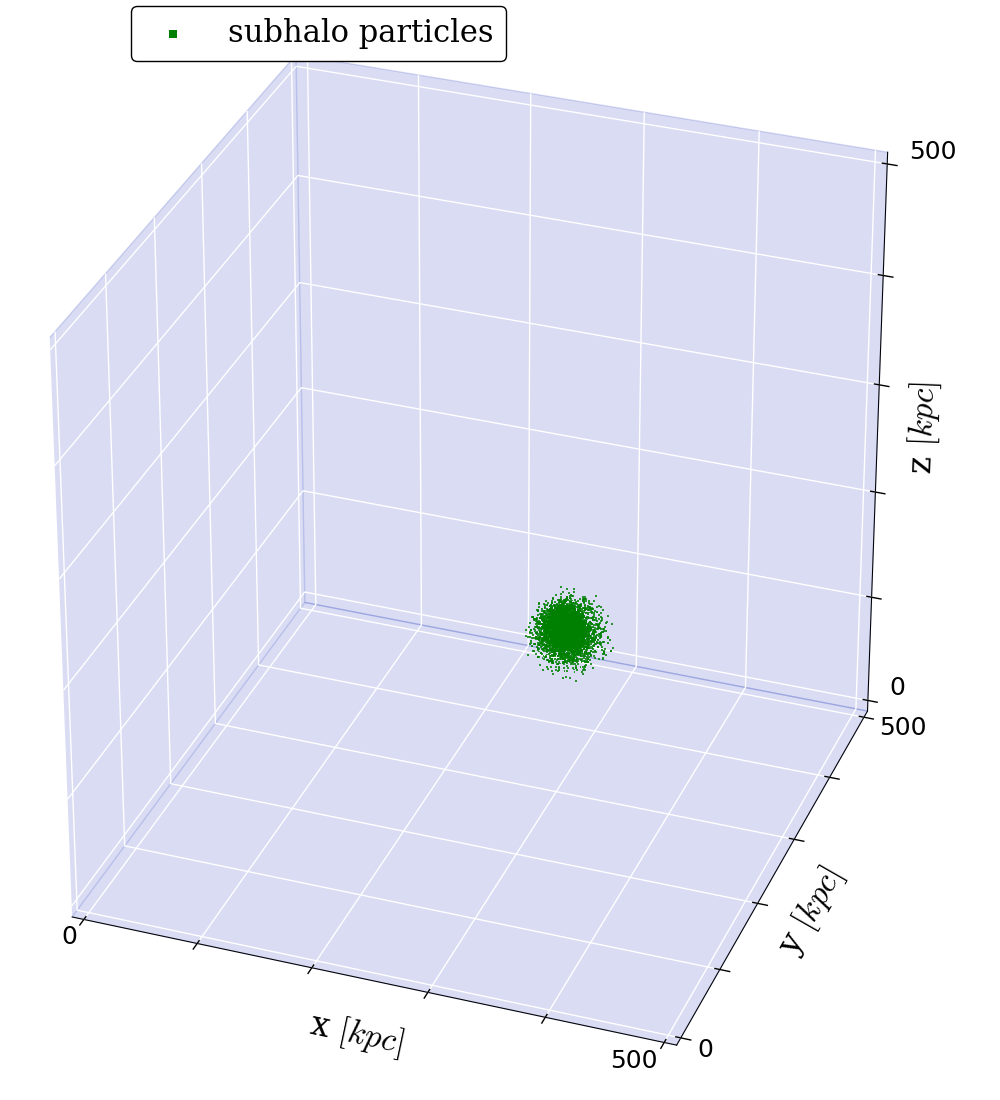
\includegraphics[width = .42\textwidth]{images/dice-two/dice-two-plot-subhalo-saddle.png}} &
			{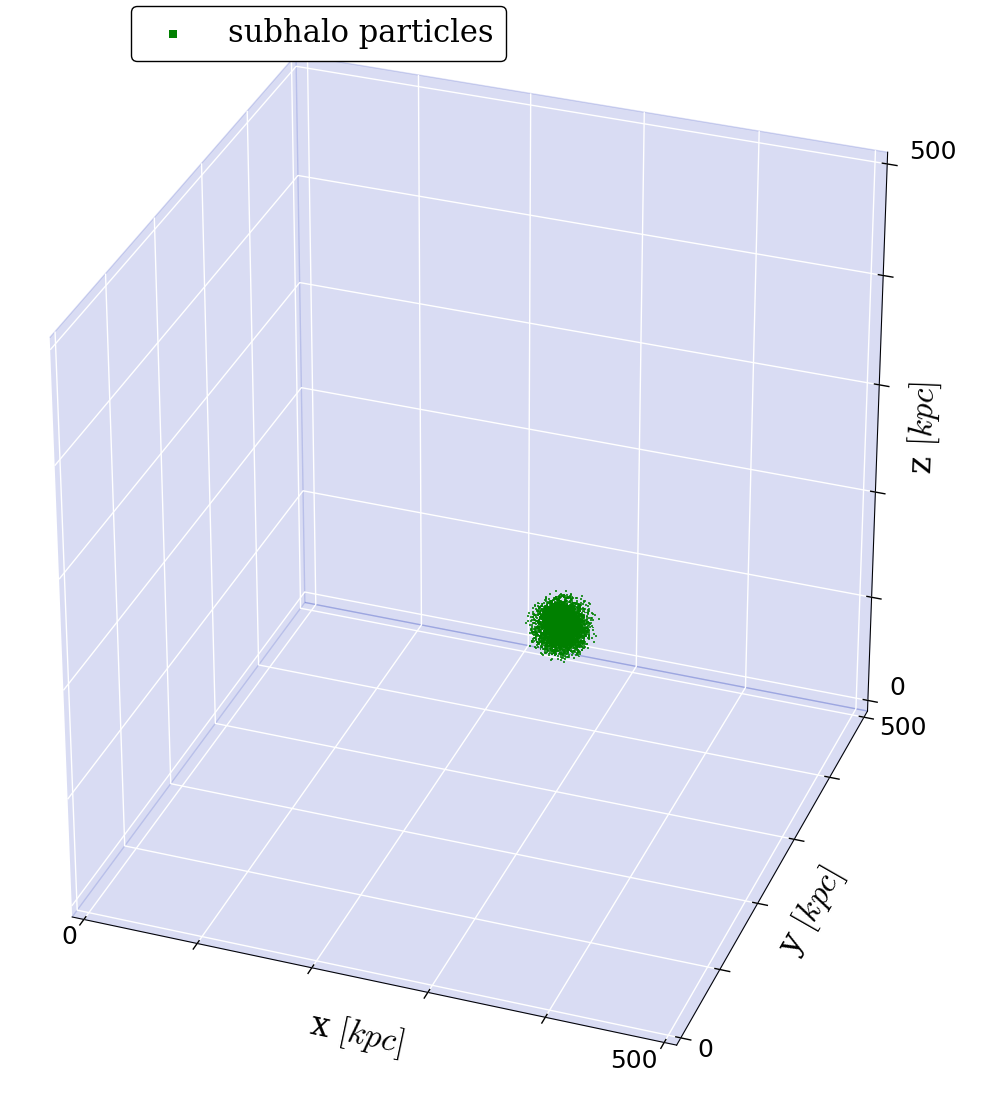
\includegraphics[width = .42\textwidth]{images/dice-two/dice-two-plot-subhalo-iter.png}} \\
			\hline
		\end{tabular}
		\caption{\label{fig:dice_two_results_b}
			The results of \neigh\ and \iter\ unbinding of the \dt-dataset: All particles, halo-namegiver particles only and subhalo particles only.
			}
		}
	\end{figure}
	\label{fig:dice_two_results}
\end{subfigures}




